%% MGT 6203 Progress Report: Group 95

\documentclass{article}
\usepackage[english]{babel}
\usepackage[utf8]{inputenc}
\usepackage{johd}
\usepackage{wrapfig}
\usepackage{tabularx}
\usepackage{enumitem}
\usepackage{hyperref}

%% ||| Title ||| %%
\title{MGT 6203 - Data Analytics for Business\\Progress Report: Team 95}

%% ||| Authors ||| %%
\author{Daniel Forcade, Ryan Hopkins, Soheil Sameti, Steven Wasserman\\

}
%% ||| Date ||| %%
\date{March 17, 2024}

\begin{document}

\maketitle

%% ||| Github Link Embedd ||| %%
\begin{center}
\textbf{Github: }{\url{https://github.gatech.edu/MGT-6203-Spring-2024-Canvas/Team-95 } }
\end{center}


%% ||| Starting Text if Needed ||| %%
%% \noindent{Rabble Rabble Rabble} 

%%%%%%%%%%%%%%%%%%%%%%%%%%%%%%%%%%%%%%%%%%%%%%
%%%% >>> Writing Section Begins Below <<< %%%%
%%%%%%%%%%%%%%%%%%%%%%%%%%%%%%%%%%%%%%%%%%%%%%

%% ||| Section 1 ||| %%                         [1]
%% ||| Background ||| %% 
\section{Background \& Problem  Statement}
\label{sec:background}
\hspace{.5cm} Weather plays a significant role in the cultivation of crops worldwide, as farmers rely on advantageous meteorological conditions to grow their crops. For years, farmers and agronomists alike have studied the weather to better understand its impacts on agricultural output, including temperature patterns, precipitation, extreme weather events, and more. The Old Farmer’s Almanac is a prime example – a comprehensive guide that recommends annual crop production periods, harvesting approaches, and more through the presentation of “astronomical data, reference charts, planting tables, weather forecasts, and more” \citep{FineGardening}.

Modern approaches to optimizing output rely on a set of practices known as precision agriculture, defined as the process of analyzing “temporal, spatial and individual plant… to support management decisions according to estimated variability for improved resource use efficiency, productivity, quality, profitability and sustainability of agricultural production” \citep{ISPA}. The collection and analysis of data to support such decision-making can illuminate dynamic weather events and processes that affect different stages of plant growth including soil erosion, nutrient deficiency, and, in cases of drought, soil salinization \citep{EOS}.

Extensive climate information at a regional level is made available to farmers through governmental organizations, similar to how you receive weather updates from your local news station. Known as a "local extension agencies," these offices offer valuable information and learning engagements for farmers, including weather and climate reports. These reports, however, cannot effectively appraise weather conditions at a level localized to individual farms or sections of a farm - think of getting a weather forecast for your home's address. The micro-climate conditions of these areas might differ significantly from regional climate forecasts, necessitating different farming practices and approaches to achieve greater success. And while farmers can collect weather data using common instruments, like affixed weather sensors that come standard with John Deere tractors \citep{JohnDeere}, functional models that take in such data and produce effectual insights are not readily available to farmers. 

\begin{wrapfigure}{r}{0.5\textwidth}
  \begin{center}
    \vspace*{-5mm}
    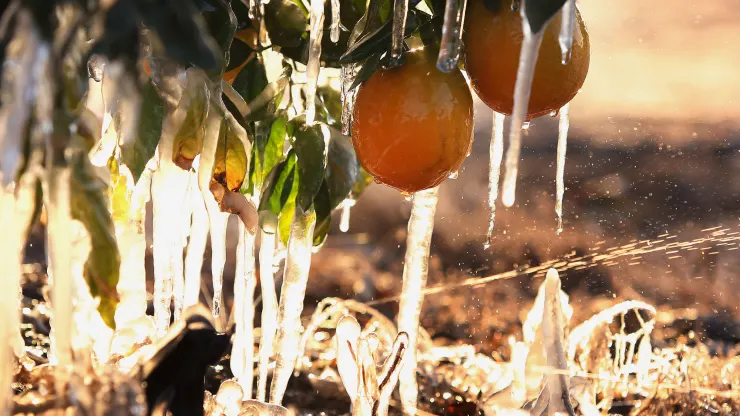
\includegraphics[width=0.45\textwidth]{Progress_Report/images/frozen_oranges.jpeg}
  \end{center}
  \vspace*{-5mm}\caption{Frozen oranges during a cold snap in December 2013 affecting the San Joaquin Valley citrus crop, in Traver, CA \citep{Orange}}
\end{wrapfigure}

This persistent issue draws an impactful business case for further research and is the topic of focus in this paper. Especially as climate change becomes more of a heightened uncertainty for the global economy, studying the effects of micro-climate weather effects on crop cultivation can aid in recommending crop growth practices to farmers and supporting the industry in sustaining resilient crop markets.

Understanding the impacts of local climate conditions at the farm level can be used to propose remediation tactics for farmers before disaster strikes. Bad weather can greatly impact the business of farming, leading to huge losses and productivity fallout. For example, seven days of freezing temperatures in 2013 led to the loss of 200,000 acres of citrus groves in California, resulting in damages amounting to \$2 billion \citep{CNBC}.

This research project aims to determine whether regional differences in climate conditions can recommend changes to crop production. The research will illuminate the correlation between climate conditions and crop yields for specified locations across the United States, and demonstrate a proof-of-concept modeling approach that can be repeated with micro-climate weather data to recommend crop production when changes to climate conditions occur.  

%% ||| Section 2 ||| %%                         [2]
%% ||| Approach ||| %% 
\section{Approach}\label{sec:approach}
\hspace{.5cm}The research project looks to analyze the climate conditions and crop yields of specified locations in the United States to identify relationships between localized weather patterns and crop yields that can be used to recommend crop production based on changing climate conditions. The research will focus on, at most, two locations of interest to validate whether the methodology is repeatable across disparate locations. Data curation will entail the collection of local-level weather data and crop production data, either at the county or ZIP code level as available. Next, data will be joined based on geospatial coordinate systems to align crop yield to direct weather conditions. Model generation will include a cadre of statistical methods, including regression to analyze cardinal temperature effects on crop production, clustering and classification to group weather conditions to crops, and cumulative sum approaches to detail weather condition changes on crop production. 

While similar approaches, such as those outlined by \citet{UIUC} and \citet{ISWS}, have performed analyses of crop production based on regional weather conditions, those researchers did not recommend approaches for using modeling with micro-climate conditions and maintained greater geographic areas of observation with their approaches. Our approach looks to collect weather data at the county or ZIP code level and relate that to crop production at the same level of observation, rather than a state or state-regional level. \citet{RemoteSens} used geospatial heatmaps of American topography to assess crop growth conditions at a county scale. Our research will operate in a similar vein, using locally measured temperature data instead of satellite infrared photography. Our approach is similar to that of \citet{Sustainability}, where several climate metrics were assessed across the Naoli River Basin in Northeast China to determine the suitability of crop production for a variety of plants. Our research, however, will not consider human factors like \citet{Sustainability} and focus exclusively on weather conditions, as it is assumed the intended users of such models would be comprised of local growers and farmers who are intimately aware of their farm's growing practices. This audience would need to be informed of approaches to incorporating insights from this research to create micro-climate models for weather conditions. A secondary audience could include federal lawmakers and employees who support federal incentives and harvest programs that can affect market conditions and promote the cultivation of specified crops. In dissenting from \citet{Sustainability}, our research would assume that human-driven decision-making could be influenced by such federal programs and market incentives. 

% This research, however, will not consider human factors, which drive the conversation of the intended audience for this research. Our team would look to promote the outcomes of this research to federal lawmakers and employees who support federal incentives and harvest programs that can affect market conditions and promote the cultivation of specified crops. For this research, then, the team will assume that human-driven decision-making could be influenced by such federal programs and market incentives. 

It should be noted that data-driven analyses such as this one are typically performed by academic institutions and corporations with the funds and resources to carry out large projects. By codifying this approach and describing the intended audience, the team looks to federate information to those without such resources and empower local growers and farmers to use this information to benefit their farming practices and respective businesses. 

%% ||| Section 3 ||| %%                         [3]
%% ||| Data Cleaning ||| %% 
\section{Data}
\hspace{.5cm}For this research effort, the process of identifying, processing, curating, and saving data is described to illuminate identified data sources, challenges with data, and key information. The data needed to support the outlined research questions includes localized weather data and localized crop yield data. The team decided to use California and Florida as test cases for the research project, given the diversity of weather patterns that occur throughout these large states. However, Vermont and Iowa were initially used to parse data from sources given their relative observed simplicity, and data was collected for these states as well. Artifacts of these states might appear in developed code. 

\subsection{Data Discovery}
\hspace{.5cm}The data needed to support the research includes localized weather data and localized crop yield data. The team reviewed several different resources online for both data domains, looking to find widely available, well-populated sources that would have the information that could best meet our needs. The primary sources the team identified and decided to use for the research are:
\begin{itemize}
    \item The USDA National Agricultural Statistics Service (NASS) Cropland Data Layer (CDL) is "an annual raster, geo-referenced, crop-specific land cover data layer produced using satellite imagery and extensive agricultural ground reference data" \citep{NASS-CDL}.
    \item The Global Surface Summary of Day (GSOD) dataset describes surface summary weather conditions, such as temperature and wind speed, for 9000 global weather stations \citep{NOAA-NCEI}. The NCEI is an office of the National Oceanic and Atmospheric Administration (NOAA).
    \item The National Climate Data Center (NCDC) Storm Events Data describes personal injuries, data estimates, and related storms recorded by county in the United States since 1950 \citep{NOAA-NCDC}. The NCDC is the world's largest climate data repository, located in Asheville, NC, and owned and operated by the National Oceanic and Atmospheric Administration (NOAA).
\end{itemize}

Crop data was initially found using George Mason University's \href{https://nassgeodata.gmu.edu/CropScape/}{CropScape} tool, an interactive GUI that shows crop yields for different counties across the United States. The GMU tool sources its data from the NASS Cropland Layer Data source that was ultimately selected. 

\subsection{Data Preparation}

\begin{wrapfigure}{l}{0.5\textwidth}
  \begin{center}
    \label{sec:raster}
    \vspace*{-8mm}
    \includegraphics[width=0.45\textwidth]{Progress_Report/images/raster_example.jpeg}
  \end{center}
  \vspace*{-5mm}
  \caption{Rendered raster image representing Carroll County in the State of Iowa, U.S. \citep{RemoteSens}}
  \vspace*{-2mm}
\end{wrapfigure}

\hspace{.5cm}After identifying each of the data sources, several preprocessing and cleaning procedures were completed to convert the data to a useable format. The datasets contained geographic location components that were in various spatial formats that could not be directly linked for analysis.  To address this, we implemented a geographic conversion and standardization pipeline that is detailed below.

The Cropland Layer Data (CDL) included crop yield for different regions using raster data, which is a gridded, pixelated data format typically associated with an identified geographical region as shown in \textbf{\hyperref[sec:raster]{Figure 2}}. This raster data was saved using Tag Image File Format (TIFF) files, the standard for storing raster image information, with each observation representing 0.22 acres of land. The raster files are compatible with ArcGIS but ill-suited for vector dataframe analysis. To solve this problem, we implemented a raster-to-vector converter utilizing \texttt{Rasterio} in Python with a EPSG:4326 geographic coordinate system. Our conversion pipeline takes in the CDL raster files for an given U.S. state, creates a descriptor column for the crop type, then refactors the EPSG:4326 spatial data into the latitude/longitude coordinates of each observation. 

The data from the conversion pipeline resulted in massive vector files that needed to be condensed. To solve this, we created a secondary pipeline that used spatial joins with additional shapefiles from the U.S. Census (\citeyear{TIGER}) to generate regions-of-interest that could be more easily matched to the weather station data. Each crop was grouped and aggregated into a summarized region, such as county or ZIP code, which significantly compressed the crop data into a manageable format for tabular analysis. This second pipeline also appended additional information from the U.S. Census data, namely land area and water area. The weather datasets initially included latitude/longitude data for each observation, which made it convenient to link to the modified crop data. Using the U.S. Census data, each weather station was matched to the regions-of-interest defined in the crop data. 

Data validation measures were taken to ensure that the data was clean and  resolute. Using data documentation from the sources, encoding was used to replace N/A values with missing flags (e.g., \texttt{-999.99} in weather) as well as  reverse-encoding binary string signifiers for weather events (e.g., \texttt{01001} into "Rain and Wind"). For later model development, a Missing at Random and Missing Completely at Random (MAR/MCAR) analysis will be used to determine imputation techniques for remediation.

Several issues arose in carrying out the data cleaning. Memory allocation issues arose with using R to perform the CDL raster conversion. The code was modified to use resolution reduction and batched parallel processing, but did not work. Instead, Python was used successfully. Another issue arose with using the Google Maps API and R package \texttt{zipcodeR} to determine a regional descriptor for each latitude/longitude observation, such as ZIP code or county. While the script worked on sample datasets, scaling up the data resulted in a slower program that could not work efficiently.

Subsets of the processed crop data and weather conditions data for California can be seen in \textbf{\hyperref[sec:cropsubset]{Figure 3}} and \textbf{\hyperref[sec:weathersubset]{Figure 4}}. Additional data elements were joined and are available for analysis, including dew point, wind gust, and more, as described in \textbf{\hyperref[sec:curated]{the appendix}}. \\

\begin{figure}[H]
\vspace*{-5mm}
\label{sec:cropsubset}
\centering
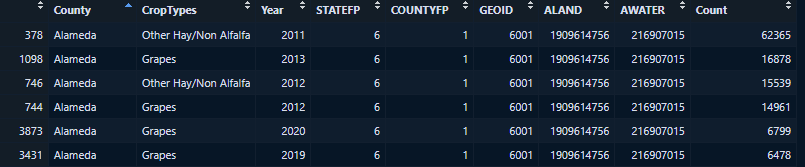
\includegraphics[width=1.0\textwidth]{Progress_Report/images/Crop_Dataset.png}
\vspace*{-5mm}
\caption{Subset of crop data for California}
\end{figure}

\begin{figure}[H]
\vspace*{-5mm}
\label{sec:weathersubset}
\centering
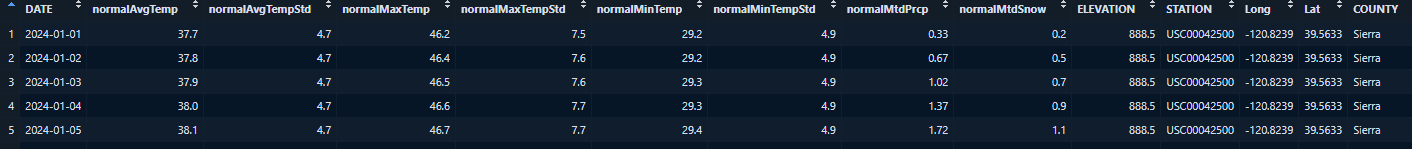
\includegraphics[width=1.0\textwidth]{Progress_Report/images/Normals_Dataset.png}
\vspace*{-5mm}
\caption{Subset of 30-yr. temperature normals for California}
\end{figure}

\subsection{Data Curation}
\hspace{.5cm}From the result set of data that was prepared, the team distilled and curated the datasets down further to better facilitate model development later on. For the crop production data, the team decided to focus on the top ten most valuable crops produced in California and Florida as part of the analysis. While the entirety of crops produced in these two states could have been kept, focusing on the top ten provides sufficient scope, simplifies analysis, and maintains the underlying intent of the research to target commonplace farming practices (which necessitates targeting the most abundant crops produced in these states and avoiding specialty crops). To accomplish this, the team used publications from the Florida Department of Agriculture and Consumer Services (\citeyear{FL-Ag}) and the California Department of Food \& Agriculture (\citeyear{CA-Ag}) to define a list of the top ten crops produced by agricultural value for each state. These lists were compared with independent sources, including \citep{Stacker}, \citep{FGS}, and \citep{FarmingWork.com}, to validate that each listing was accurate and widely -accepted. Filters were applied in R using observations on the representational descriptor variables, then data was split and saved off. The selected crops for California and Florida are available in \textbf{\hyperref[sec:choices]{the appendix}}.

Once set, the team stored the data as CSVs in Github. These datasets can be easily queried for further development later in the project, and describe the data necessary to answer the outlined research questions. Descriptions of the available data can be reviewed in \textbf{\hyperref[sec:curated]{the appendix}}.

%% ||| Section 4 ||| %%                         [4]
%% ||| Models ||| %% 
\section{Initial Insights \& Next Steps}

\subsection{Initial Model Creation}
\hspace{.5cm}While more extensive model development is planned as part of the next phase of the research project, several models were created to describe average weather observations in California. This included annual progressions of the mean and deviation of daily average temperature, daily minimum temperature, and daily maximum temperature over the 30 years of data available, as shown in \textbf{\hyperref[sec:dataviz1]{Figure 5}}. Additionally, the average month-to-date precipitation and snowfall for the 30-year observational period are also shown. Further model development is described in \textbf{\hyperref[sec:approach]{the planned approach}}.

A cumulative sum (CUSUM) model was also created to determine critical change detection of temperature observations in the dataset, with outputs depicted in \textbf{\hyperref[sec:dataviz2]{Figure 6}}. The idea is to establish an effective threshold for monitoring future observations and ascertain whether this threshold changes based on crop type, location, or any other independent variable available in the data. Initial experimentation with this model has begun, but has not yielded reportable results yet. \\

\begin{figure}[H]
\label{sec:dataviz1}
\begin{tabular}{cc}
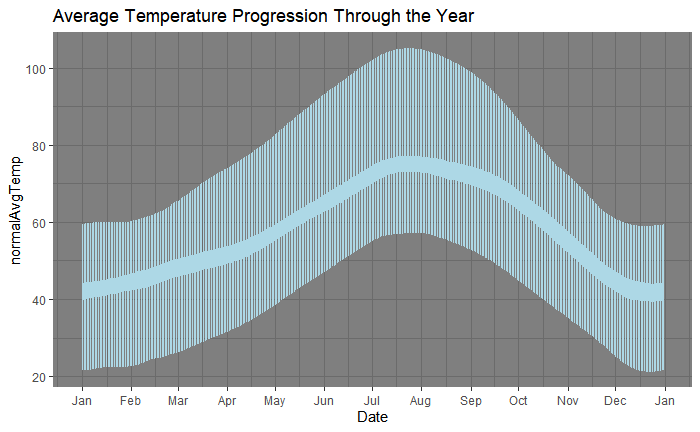
\includegraphics[width=0.5\textwidth]{Progress_Report/images/AvgTemp_avg.png} &
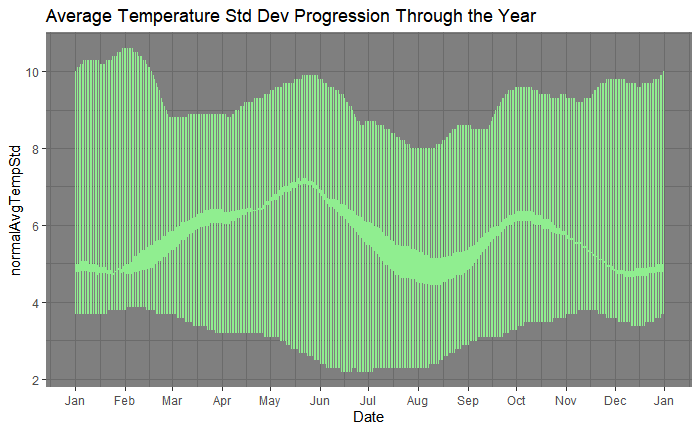
\includegraphics[width=0.5\textwidth]{Progress_Report/images/AvgTemp_std.png} \\
% 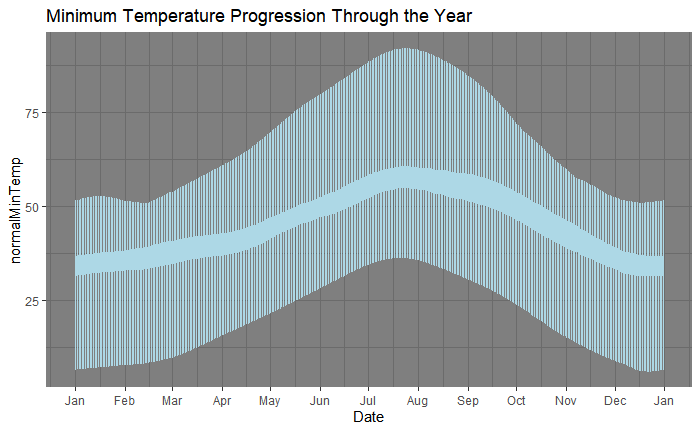
\includegraphics[width=0.5\textwidth]{Progress_Report/images/MinTemp_avg.png} &
% 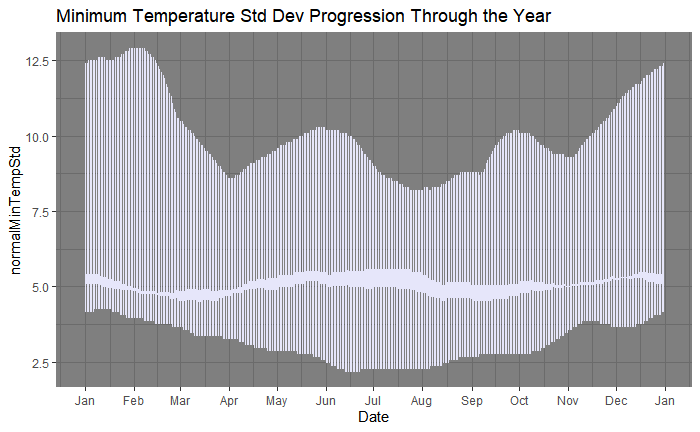
\includegraphics[width=0.5\textwidth]{Progress_Report/images/MinTemp_std.png} \\
% 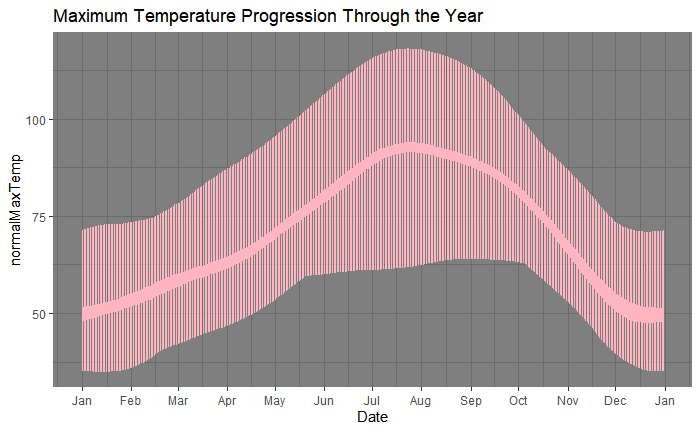
\includegraphics[width=0.5\textwidth]{Progress_Report/images/MaxTemp_avg.png} &
% 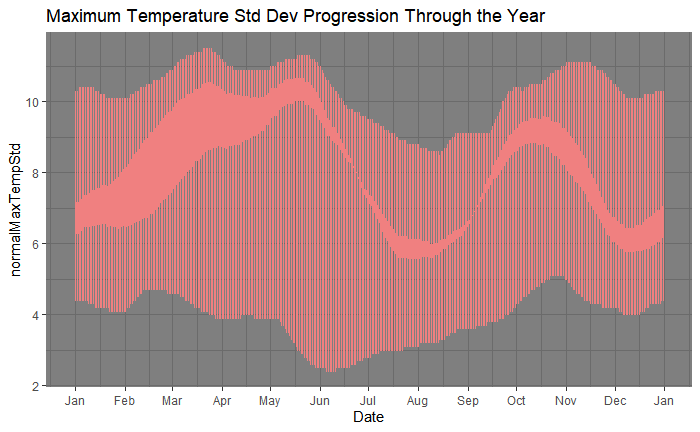
\includegraphics[width=0.5\textwidth]{Progress_Report/images/MaxTemp_std.png} \\
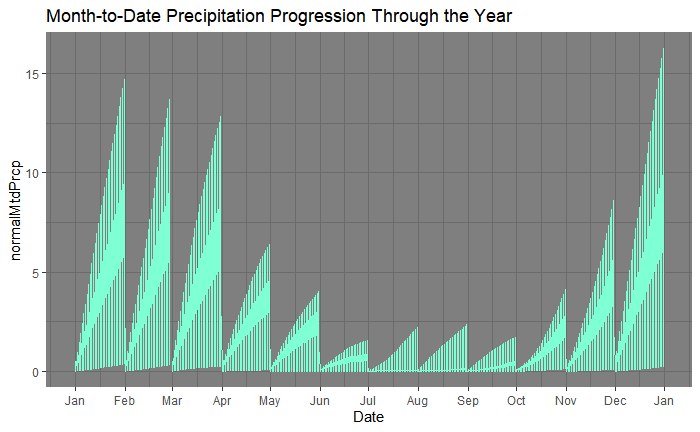
\includegraphics[width=0.5\textwidth]{Progress_Report/images/MTDPrecipitaion_avg.png} &
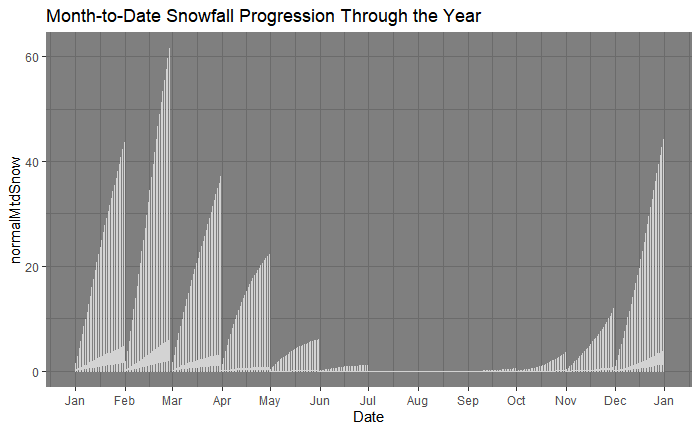
\includegraphics[width=0.5\textwidth]{Progress_Report/images/MTDSnowfall_avg.png} \\
\end{tabular}
\vspace*{-5mm}
% \caption{Annual progressions of average, minimum, and maximum temperature, Precipitation, and Snowfall data in California for a 30-year observational period.}
\caption{Annual progression of daily-average temperature mean and deviation; average precipitation, and average snowfall in California over 30-year observational period.}
\end{figure}

\begin{figure}[H]
\vspace*{-5mm}
\label{sec:dataviz2}
\centering
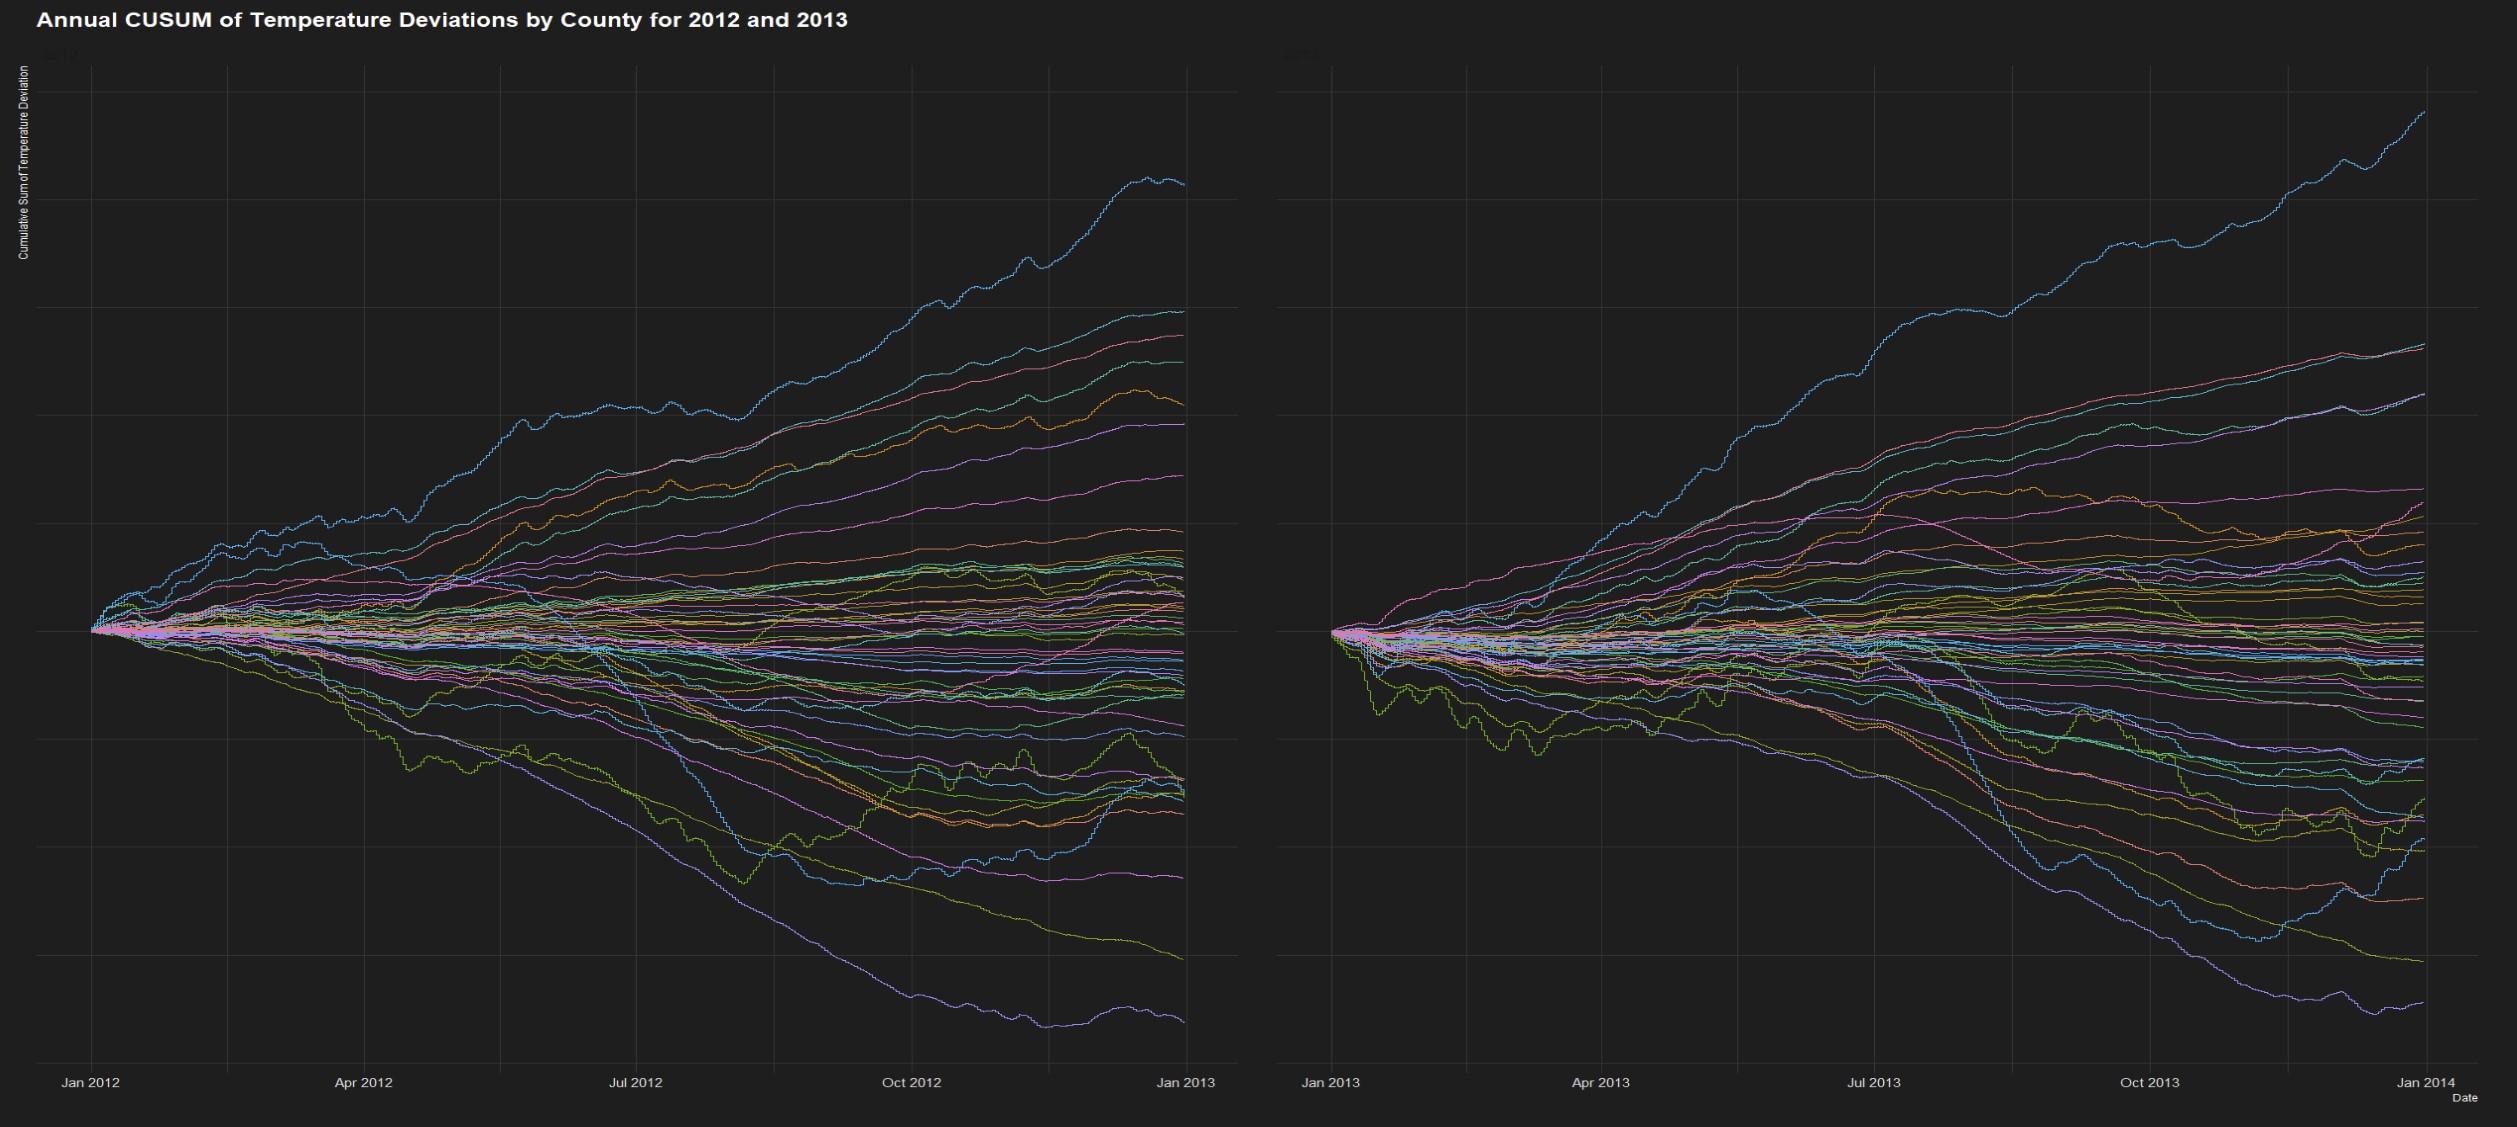
\includegraphics[width=1.0\textwidth]{Progress_Report/images/CUSUM_2.jpg}
\vspace*{-5mm}
\caption{Cumulative sum (CUSUM) models for average daily temperatures in 2012 and 2013 compared to 30-yr. temperature normals in California counties}
\end{figure}

\subsection{Planned Model Development}
\hspace{.5cm}Continued model development requires the establishment of initial thresholds for CUSUM and other models. The team sought to identify a source that could describe baseline expectations for temperature ranges that different crops thrive in. In horticulture, this concept is known as \textit{cardinal temperatures} - namely, the minimum, maximum, and optimum temperature ranges for different crops. Using the research established by \citep{Horticulturae}, the team will look to develop models that align to the given temperature ranges for each crop, discern historical incidents where the model would suggest threats to plant health, and then ascertain whether those flagged incidents would lead to actual damages. One example of this workflow would include evaluating historical temperatures in the San Joaquin Valley part of the California study and see whether the model would flag December 2013, which would align with the business case sample described by \citep{CNBC}, which was outlined in \hyperref[sec:background]{the problem background}.

From here, further models can be created using regression to determine plant preferences for climate conditions, and eventually, start and stop months for crop production and harvesting. The outputs of these models can be compared with observational data found in literature or anecdotal information shared directly by farmers and growers. Additionally, a risk model can be created using classification and clustering models to determine which counties in each state are at risk given changing climate conditions, and a recommendation system built to recommend changes to crops produced, harvesting times, and more. 

\subsection{Timeline Reporting}
\hspace{.5cm}It should be noted that the final report is ahead of schedule to be completed by the final deliverable due date. The next phase of the work includes model development and synthesis, for which preliminary work has been completed. In terms of the project timelines, the team is ahead of the schedule originally set out in \href{{https://github.gatech.edu/MGT-6203-Spring-2024-Canvas/Team-95/blob/8e0b617b8c53ad76f4974ec25019710f2ce385cc/Project%20Proposal/team095proposal.pdf}}{the project proposal}.

%%%%%%%%%%%%%%%%%%%%%%%%%%%%%%%%
%% ||| Section References ||| %%                           [B]
%%%%%%%%%%%%%%%%%%%%%%%%%%%%%%%%
%% Imported autoformating for References in the bib.bib file
%% References can be put into there and it should automatically format.  If issues we can build our own.

\bibliographystyle{johd}
\bibliography{bib}

%%%%%%%%%%%%%%%%%%%%%%%%%%%%%%%%

\appendix
\section{Appendix}
\subsection{Curated Data}
\label{sec:curated}
The following datasets were curated, stored in the Github repository, and are ready for further analysis. 

\begin{itemize}[noitemsep]
    \item Crop Data by County, Mapped and Aggregated - California and Florida, 2010-2020
    \item 30-Year Normals by County, Mapped - California and Florida, 1991-2020
    \begin{itemize}[noitemsep]
        \item Average, Minimum, and Maximum Temperatures - Point Estimates and STD.DEVs
        \item Month-to-Date (MTD) Snow and Rain - Point Estimates
    \end{itemize}
    \item 30-Year Normals by Weather Station, Mapped - California and Florida, 1991-2020
    \item Daily Weather by County - California and Florida, 2010-2020
    \begin{itemize}[noitemsep]
        \item Dew Point
        \item Wind Gust / Max Wind Speed / 5 Min Wind Speed High
        \item Max Temp / Min Temp / Avg Temp
        \item Precipitation
        \item Elevation
        \item One-Hot Encoding for Basic Weather Event: Fog/Ran/Snow/Hail/Thunder/Tornado
    \end{itemize}
\end{itemize}

% NOTE: I originally wrote this to be a data dictionary - gonna save it for later. PLEASE DON'T DELETE - THANKS!

% \subsection{Table 1 Name here}

% This table describes ... \\

% \begin{tabularx}{1.0\textwidth} { 
%   | >{\raggedright\arraybackslash}X 
%   | >{\raggedright\arraybackslash}X | }
%  \hline
%  \textbf{Data Element} & \textbf{Data Definition} \\
%  \hline
%  1  & ABC  \\
% \hline
% \end{tabularx}

% \subsection{Table 2 Name here}

% This table describes ... \\

% \begin{tabularx}{1.0\textwidth} { 
%   | >{\raggedright\arraybackslash}X 
%   | >{\raggedright\arraybackslash}X | }
%  \hline
%  \textbf{Data Element} & \textbf{Data Definition} \\
%  \hline
%  1  & ABC  \\
% \hline
% \end{tabularx}

\subsection{Crop Choices}
\label{sec:choices}

This section describes the ten crops selected for observation in California and Florida. \\

\begin{tabularx}{1.0\textwidth} { 
  | >{\raggedright\arraybackslash}X 
  | >{\raggedright\arraybackslash}X | }
 \hline
 \textbf{California} & \textbf{Florida} \\
 \hline
 1. Rice  & 1. Corn  \\
 2. Other Hay/Non Alfalfa  & 2. Potatoes  \\
 3. Tomatoes  & 3. Sugarcane  \\
 4. Grapes  & 4. Watermelons  \\
 5. Almonds  & 5. Tomatoes  \\
 6. Walnuts  & 6. Citrus  \\
 7. Pistachios  & 7. Oranges  \\
 8. Oranges  & 8. Peppers  \\
 9. Strawberries  & 9. Strawberries  \\
 10. Lettuce  & 10. Blueberries  \\ 
\hline
\end{tabularx}

% \textbf{California}
% \begin{itemize}[noitemsep]
%     \item[1.] Rice
%     \item[2.] Other Hay/Non Alfalfa
%     \item[3.] Tomatoes
%     \item[4.] Grapes
%     \item[5.] Almonds
%     \item[6.] Walnuts
%     \item[7.] Pistachios
%     \item[8.] Oranges
%     \item[9.] Strawberries
%     \item[10.] Lettuce
% \end{itemize}

% \textbf{Florida}
% \begin{itemize}[noitemsep]
%     \item[1.] Corn
%     \item[2.] Potatoes
%     \item[3.] Sugarcane
%     \item[4.] Watermelons
%     \item[5.] Tomatoes
%     \item[6.] Citrus
%     \item[7.] Oranges
%     \item[8.] Peppers
%     \item[9.] Strawberries
%     \item[10.] Blueberries
% \end{itemize}

\end{document}